%
% flow design
%

\documentclass[12pt]{article} % FORMAT CHANGE
\usepackage[dvips]{graphicx}
\usepackage{times}

\graphicspath{{./}{figs/}} 

%
% GET THE MARGINS RIGHT, THE UGLY WAY
%
% \topmargin 0.2in
% \textwidth 6.5in
% \textheight 8.75in
% \columnsep 0.25in
% \oddsidemargin 0.0in
% \evensidemargin 0.0in
% \headsep 0.0in
% \headheight 0.0in

\pagestyle{plain}

\addtolength{\hoffset}{-2cm}
\addtolength{\textwidth}{4cm}

\addtolength{\voffset}{-1.5cm}
\addtolength{\textheight}{3cm}

\setlength{\parindent}{0pt}
\setlength{\parskip}{12pt}

\title{Flow Design Document}
\author{PVFS Development Team}
\date{July 2002}

\begin{document}

\maketitle

\section{Concepts and Motivation}

Flows are a high level model for how PVFS2 system components
will perform I/O.  It is designed to abstractly but efficiently move
data from source to destination, where source and destination may be
defined as storage devices, network devices, or memory regions.

Here are some features:

\begin{itemize}

\item \emph{Combining I/O mechanisms}  The flow interface combines
network I/O and disk I/O into a coherent framework.  This lets us
make scheduling decisions that take both into account.

\item \emph{Support for different protocols}
Actual I/O is carried out underneath the flow interface by
\emph{flow protocols}.   We may implement several different
protocols (using different I/O or buffering techniques, for example)
which can be switched out without modifying the API.

\item \emph{Simple interface}  The application interface to
this system will be as high level and simple as possible.  Device
selection, scheduling, buffer management, and request pattern
processing will be transparent to the flow user.  

\end{itemize}

\section{Related documents}

\begin{itemize}
\item pvfs2-design-bmi: outlines the BMI interface, which is a low
level networking component used by the default flow protocol
\item pvfs2-design-storageint: outlines the Trove interface, which
is a low level byte stream and key/value storage interface used by
the default flow protocol
\item pvfs2-design-concepts: general PVFS2 definitions and overview
\item pvfs2-design-request: covers the distribution and I/O
request language interfaces
\item pvfs2-design-job: covers the high level glue layer that
pulls the flow, BMI, trove, and scheduling interfaces together
into a unified API for managing pending operations.
\end{itemize}

\section{Flows}

\subsection{Overview}

A flow describes a movement of data.  The data always moves from a single
source to a single destination.  There may be (and almost always will be)
multiple flows in progress at the same time for different locations-
in particular for clients that are talking simultaneously to several
servers, or servers that are handling simultaneous I/O requests.

At the highest level abstraction, it is important that a flow describes
a movement of data in terms of ``what to do'' rather than ``how to do
it''.  For example, when a user sets up a flow, it may indicate that the
first 100 bytes of a file on a local disk should be sent to
a particular host on the network.  It will not specify what protocols to
use, how to buffer the data, or how to schedule the I/O.  All of this will be
handled underneath the flow interface.  The user just requests that a
high level I/O task be performed and then checks for completion until it
is done.

Note that the ``user'' in the above example is most likely a
system interface or server implementer in pvfs2.  End users will
be unaware of this API.

A single flow created on a server will match exactly one flow on a
client.  For example, if a single client performs a PVFS2 read, the
server will create a storage to network flow, and the client will
create a network to memory flow.

Flows will not be used for exchanging request protocol messages
between the client and server (requests or acknowledgements).
Flows will be used exclusively for data transfer during I/O
operations.

Flows allow the user to specify the on disk data layout
(distribution) as well as complex I/O request patterns (similar to
MPI datatypes) for I/O operations.  The flow interface will
interact with the request processing and distribution subsystems
of PVFS2 to interpret these patterns.

\subsection{Architecture}
\label{sec:arch}

There are two major parts of the flow architecture, as seen in figure
\ref{fig:flow-arch}.  The first is the
\emph{flow interface}.  Applications (ie PVFS components) interact with
this interface.  It provides a consistent API regardless of what
protocols are in use, what scheduling is being performed, etc.  

The second major component of the architecture is the \emph{flow
protocol}.
There may be many flow protocols active within one flow interface.  Each
flow protocol implements communication between a different pair of data
endpoint types.  For example, one flow protocol may link TCP/IP to
asynchronous unix I/O, while another may link VIA to memory regions.  For
two seperate hosts to communicate, they must share compatible flow
protocols (as indicated by the dotted line at the bottom of figure
\ref{fig:flow-arch}).

Flow protocols all adhere to a strict interface 
and must provide the same expected functionality (all of which will be
described later).  Flow protocols take care of details such as buffering
and flow control if necessary.


\begin{figure}
\begin{center}
\caption{Basic flow architecture \label{fig:flow-arch}}
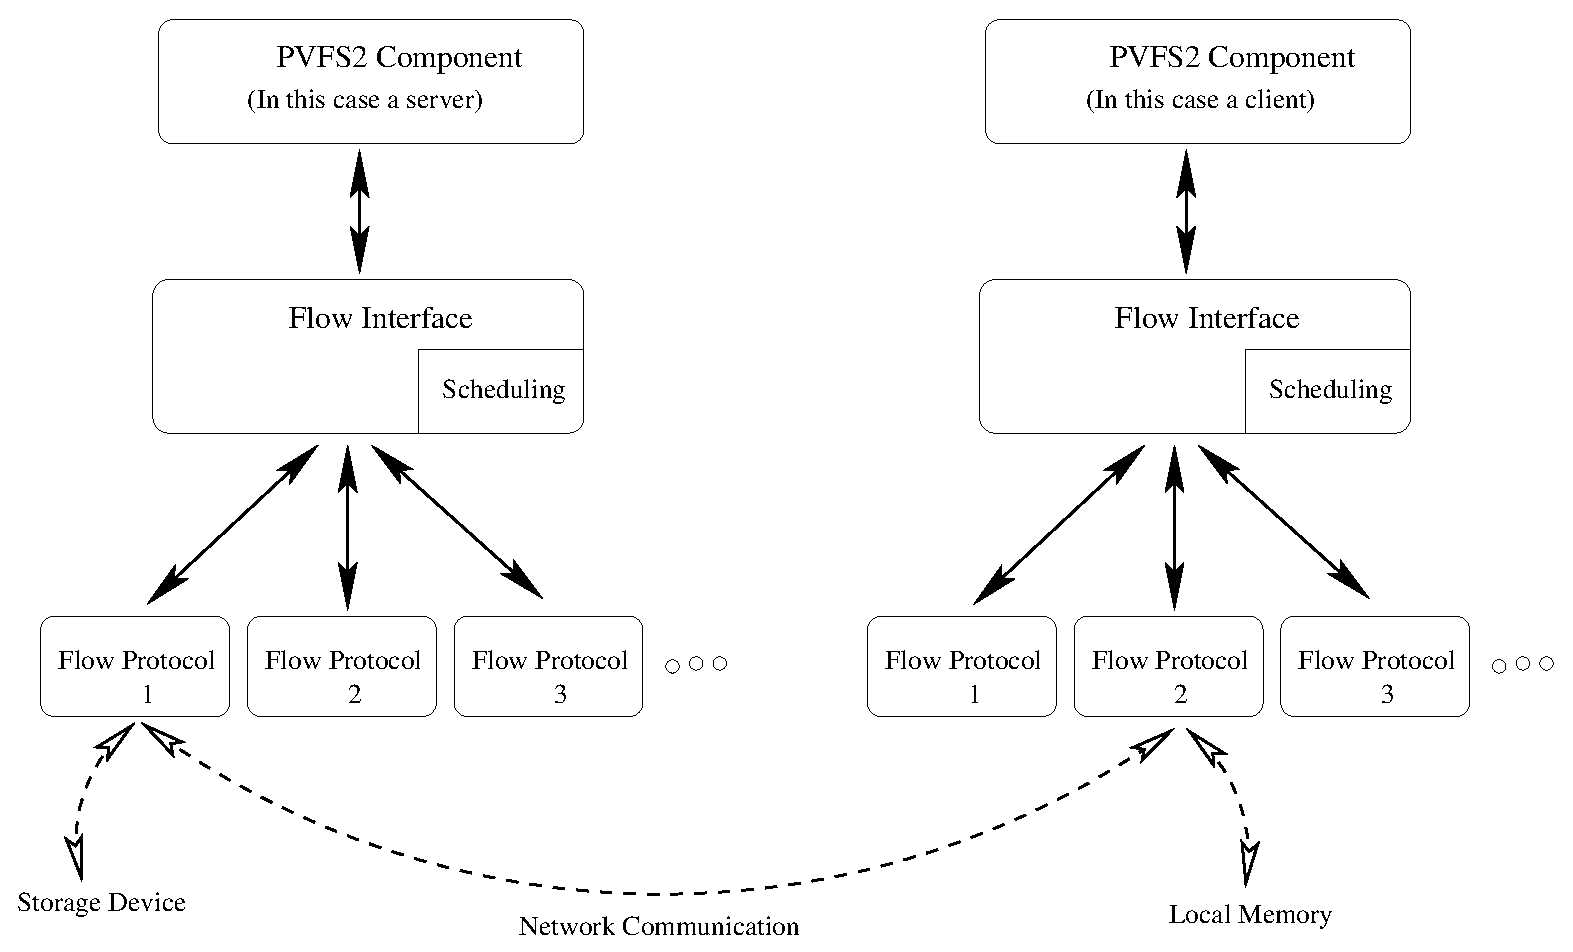
\includegraphics[scale=0.6]{flow-arch.eps}
\end{center}
\end{figure}

\subsection{Describing flows}

Individual flows are represented using structures called \emph{flow
descriptors}.  The source and destination of a given flow are represented
by structures called \emph{endpoints}.  A flow descriptor may serve
many roles.  First of all, when created by a flow interface user, it
describes an I/O task that needs to be performed.  Once it is submitted
to the flow interface, it may keep up with state or progress information.
When the descriptor is finally completed and returned to the user, it will
indicate the status of the completed flow, whether successful or in error.

Flow endpoints describe the memory, storage, or network locations for
the movement of data.  

\subsection{Usage assumptions}

It is assumed that all flows in PVFS2 will be \emph{preceded} by a
PVFS2 request protocol exchange between the client and server.  In
a file system read case, the client will send a read request, and
the server will send an acknowledgement (which among other things
indicates how much data is available to be read).  In a file
system write case, the client will send a write request, and the
server will send an acknowledgement that indicates when it is safe
to begin the flow to send data to the server.

If a flow ends processing early, or completes in error, it can be
assumed that the flow will be followed by a request protocol
echange that indicates what error was encountered.  The flows do
not exchange error information on their own.

An important side effect of this model is that the flow interface
should always know in advance how much data should be transfered
on both the client and the server side.  If less data is
transmitted, then it may be considered an error condition.  This
essentially means that the flow interface is not responsible for
detecting and handling EOF on read operations.

The request protocol will be responsible for transmitting any file
size or other information needed by the request processing
components.

\section{Data structures}

\subsection{Flow descriptor}
\label{sec:flow-desc}

Flow descriptors are generally created manually by the flow interface
user.  At this time, the caller may edit these fields directly.  Once the
flow has been posted for service, however, the caller may only interact
with the descriptor through functions defined in the flow interface.
It is not safe to directly edit a flow descriptor while it is in progress.

Once a flow is complete, it is again safe to examine fields within
the descriptor (for example, to determine the status of the
completed flow).

Note that there is an endpoint specific to each type supported by
the flow interface (currently memory, BMI (network), and Trove
(storage)).

\begin{verbatim}

struct flow_descriptor
{
   /**********************************************************/
   /* fields that can be set publicly before posting */

   struct flow_endpoint src;  /* src endpoint */
   struct flow_endpoint dest; /* dest endpoint */
   int flags;       /* optional flags */
   PVFS_msg_tag_t tag;         /* matching tag */
   void* user_ptr;            /* for use by caller */
   PINT_Request* request;     /* I/O request description */
   /* information about the file that we are accessing */
   PINT_Request_file_data* file_data;  

   /***********************************************************/
   /* fields that can be read publicly upon completion */

   int state;        /* final state of flow */
   PVFS_error error_code;      /* specific errno value if failure */
   PVFS_size total_transfered; /* total amt. of data xfered */

   /***********************************************************/
   /* fields reserved strictly for internal use */

   int flowproto_id;           /* identifies which protocol owns this */
   int priority;     /* priority of this flow */
   struct qlist_head sched_queue_link;  /* used by scheduler */
   void* flow_protocol_data;   /* used by flow protocols */
   PINT_Request_state* request_state;   /* req processor state */
   PVFS_offset current_req_offset; /* offset of request processing */
   PVFS_offset* offset_array;  /* array of offsets being processed */
   PVFS_size* size_array;      /* array of sizes being processed */
};
typedef struct flow_descriptor flow_descriptor;


/* describes BMI endpoints */
struct BMI_endpoint_data
{
   bmi_addr_t address;
};

/* describes trove interface endpoints */
struct trove_endpoint_data
{
   PVFS_coll_id coll_id;
   PVFS_handle handle;
};

/* describes memory region endpoints */
struct mem_endpoint_data
{
   void* buffer;
   PVFS_size size;
   int prealloc_flag;
};

struct flow_endpoint
{
   PVFS_endpoint_type endpoint_id;
   union
   {
      struct BMI_endpoint_data bmi;
      struct trove_endpoint_data trove;
      struct mem_endpoint_data mem;
   } u;
};
typedef struct flow_endpoint flow_endpoint;

\end{verbatim}

\section{Avoiding flows}

The flow interface will introduce overhead for small operations
that would not otherwise be present.  It may therefore be helpful
to eventually introduce an optimization to avoid the use of flows
for small read or write operations.

\begin{verbatim}

text of an email discussion on this topic (> part by Phil, non >
part by Rob):

> Yeah, we need to get these ideas documented somewhere.  There may actually
> be a couple of eager modes.  By default, BMI only allows unexpected
> messages < 16K or so.  That places a cap on the eager write size,
> unless we had a second eager mode that consists of a) send write request
> b) send write data c) receive ack...

Yes.  These two modes are usually differentiated by the terms "short" and
"eager", where the "short" one puts the data actually into the same
packet/message (depending on the network layer at which we are working).

> Of course all of this would need to be tunable so that we can see what
> works well.  Maybe rules like:
> 
> contig writes < 15K : simple eager write
> 15K < contig writes < 64K : two part eager write
> writes > 64K && noncontig writes : flow
> 
> contig reads < 64K : eager read
> contig reads > 64K && noncontig reads : flow

Yeah, something like that.

\end{verbatim}

\section{Flow interface}

The flow interface is the set of functions that the flow user is allowed
to interact with.  These functions allow you to do such things as create
flows, post them for service, and check for completion.

\begin{itemize}
	\item \emph{PINT\_flow\_initialize()}: performs initial setup of flow
	interface - must be called before any other flow interface functions
	\item \emph{PINT\_flow\_finalize()}: shuts down the flow interface
	\item \emph{PINT\_flow\_alloc()}: creates a new flow descriptor
	\item \emph{PINT\_flow\_free()}: frees up a flow descriptor that is
	no longer needed
	\item \emph{PINT\_flow\_reset()}: resets a previously used flow
	descriptor to its initial state and values.
	\item \emph{PINT\_flow\_set\_priority()}: sets the priority of a
	particular flow descriptor.  May be called even when a flow is in
	service.
	\item \emph{PINT\_flow\_get\_priority()}: reads the priority of a
	particular flow descriptor.  May be called even when a flow is in
	service.
	\item \emph{PINT\_flow\_post()}: submits a flow descriptor for
	service
	\item \emph{PINT\_flow\_unpost()}: aborts a previously posted flow
	\item \emph{PINT\_flow\_memalloc()}: allocates a memory region that
	is optimized for use with a particular type of flow.
	\item \emph{PINT\_flow\_memfree()}: releases a memory region that was
	previously allocated with \emph{PINT\_flow\_memalloc}
	\item \emph{PINT\_flow\_setinfo()}: used to set optional
	interface parameters.
	\item \emph{PINT\_flow\_getinfo()}: used to read optional
	interface parameters.
\end{itemize}

There are two sets of functions provided for testing of completion of
flows.  The functions in the first set must return immediately.  They are
intended as a very quick check for completion without doing any work.
Note that these functions should \emph{not} be called repeatedly within
a small service loop, because that would waste CPU cycles in a busy spin
that doesn't really do anything productive.

\begin{itemize}
	\item \emph{PINT\_flow\_test()}: tests for completion of a particular
	flow
	\item \emph{PINT\_flow\_testsome()}: tests for completion of any
   flows from a specified set of flows
	\item \emph{PINT\_flow\_testworld()}: tests for completion of any
	flows that are in service in the interface 
\end{itemize}

The second set of functions are allowed to do a bounded amount of work
during each invocation.  They will not block indefinitely, but may
briefly hold program control.  These functions may be safely used
within tight service loops.

\begin{itemize}
	\item \emph{PINT\_flow\_wait()}: tests for completion of a particular
	flow
	\item \emph{PINT\_flow\_waitsome()}: tests for completion of any
	flows from a specified set of flows
	\item \emph{PINT\_flow\_waitworld()}: tests for completion of any
	flows that are in service in the interface
\end{itemize}

\section{Flow protocol interface}

The flow protocols are modular components capable of moving data between
\emph{particular} types of endpoints.  (See section \ref{sec:arch} for an
overview).  Any flow protocol implementation must conform to a
predefined flow protocol interface in order to interoperate with the
flow system.  

\begin{itemize}

	\item \emph{flowproto\_initialize()}: Initializes the flow
	protocol
	\item \emph{flowproto\_finalize()}: shuts down the flow
	protocol (forceful terminating any pending flows)
	\item \emph{flowproto\_memalloc()}: allocates a region of
	memory optimized for use with the flow protocol
	\item \emph{flowproto\_memfree()}: frees up memory regions
	previously allocated with \emph{flowproto\_memalloc}
	\item \emph{flowproto\_announce\_flow()}:
	\item \emph{flowproto\_check()}: check to see if a particular
	flow is ready for service
	\item \emph{flowproto\_checksome()}: check to see if any flows
	from a specified set of flows is ready for service
	\item \emph{flowproto\_checkworld()}: check to see if any
	active flows
	\item \emph{flowproto\_service()}: performs work on a single
	flow descriptor that is ready for service (as indicated by a
	flowproto check function)
	\item \emph{flowproto\_getinfo()}: reads optional parameters
	from the protocol
	\item \emph{flowproto\_setinfo()}: sets optional protocol
	parameters
\end{itemize}

\section{Inner workings of the flow interface (implementation)}

The flow interface contains the \emph{flow service loop}, which drives
the work being done within the flow system.  It operates above the flow
protocols, and handles overall scheduling and processing of active flows.
Note: this service loop is currently implemented internally in the
\emph{do\_one\_work\_cycle()} function.  It is only activated
during PINT\_flow\_waitXXX() calls, as the flow interface does not
posess its own thread of control.

The flow interface maintains four seperate queues to track flows
that are in progress:

\begin{itemize}
\item completion\_queue: holds completed flow descriptors until
they are returned to the caller through a test or wait function.
\item transmitting\_queue: holds flow descriptors that are
currently transmitting data (either to/from network or disk).
\item need\_svc\_queue: holds flow descriptors that have done as
much transmitting as they can in their current state.  These flows
are ready to be serviced by the flowproto\_service() function so
that they may continue.
\item scheduled\_queue: holds flow descriptors that were
previously kept in the need\_svc\_queue but have been chosen by
the scheduler to actually be serviced.
\end{itemize}

The flow service loop operates as follows:

\begin{enumerate}
	\item The flow service loop will first run
	\emph{flowproto\_checkworld()} for each active flow protocol to
	determine which ones are ready for service.
	\item A scheduling and priority filter is applied to the set of flows
	that are ready for service.  This will produce an ordered subset that
	have been scheduled for service.
	\item The resulting scheduled flows are then serviced one at a time, in
	order.  This is done by calling the \emph{PINT\_flowproto\_service}
	from the appropriate protocol for each flow.  Flows are then
	added back to the appropriate queues depending on the result.
	\item Goto step 1.
\end{enumerate}

The scheduling and priority filter will be modular so that it can be
replaced or modified without reworking the overall flow service loop.
The default scheduler simply schedules every flow that is ready
for service in the order that they arrive.  NOTE: this is
implemented internally in the default\_scheduler() function.

\subsection{Default flow protocol (implementation)}

The default flow protocol will use BMI and Trove for all I/O
operations.  It will be capable of handling the following endpoint
pairs:

\begin{itemize}
\item BMI to memory 
\item memory to BMI
\item BMI to Trove
\item Trove to BMI
\end{itemize}

As of this writing, Trove endpoint handling is not yet
implemented.

The BMI to memory and memory to BMI flows are relatively simple.
A default buffer size will be chosen for all BMI operations.  Thus
memory to BMI transfers will simply consist of a series of BMI
send operations until the entire region has been transferred.
Memory to BMI transfers will consist of a series of BMI receives
until the data region has been filled.

The flows that involve both BMI and Trove are slightly more
complex.  For this type of flow to work, data must be transfered
to an intermediate buffer between BMI and Trove.  The default flow
protocol does this through double buffering, so that one buffer
can be emptied while the other is filling.  This allows both Trove
and BMI to operate simultaneously on the same flow.

The flow protocol maintains three internal queues.  One is for BMI
operations that are in flight, one is for Trove operations that
are in flight, and one is for flows that are either completed or
ready for service (to be returned to the flow interface during a
checkXXX() call).

\subsubsection{checkworld() (implementation)}

The checkworld function begins by building arrays of pending BMI
and Trove operations.  It then tests BMI and Trove to determine if
any of them have completed.  Each completed BMI or Trove operation
is then mapped back to the flow that it belongs to (using user
pointers).  The flow state is then modified (the flow may have
completed, it may be ready for service, or it may remain in its
current state pending the completion of another operation).

\subsubsection{handling BMI to memory flows (implementation)}

No double buffering is performed in this case.  

The amount of data to transfer at each step is limited by the buffer
size used by the flow protocol.  Also note that there is a limit to
the number of discontiguous regions that the flowprotocol is willing to
handle with a single BMI operation.

At each step, the PINT\_process\_request() function is called to determine
what memory regions should be filled by the operation.  Assuming
that the number of resulting discontiguous regions does not exceed
a predefined maximum, a BMI list receive operation is posted to
transfer the next message directly into the desired memory
regions.

If the maximum number of discontiguous regions per step is
exceeded, however, an intermediate buffer is created and the next
message is received into a contiguous region.  memcpy() is then
used to copy each discontiguous region into its final memory
location.  Intermediate buffers are non released until the flow
has completed (in case it can be used in more than one step of the
transfer).

Short BMI receives are tolerated, because they may simply indicate
that the sender was not able to send as much data as was desired
in this step.  If a short receive occurs, future processing simply picks
back up where the receive left off.

If a zero byte BMI message is received, that indicates that the
sender encountered a problem that prevented it from continuing.
The flow should be aborted at this point.

\subsubsection{handling memory to BMI flows (implementation)}

No double buffering is performed in this case.  

The amount of data to transfer at each step is limited by the buffer
size used by the flow protocol.  Also note that there is a limit to
the number of discontiguous regions that the flowprotocol is willing to
handle with a single BMI operation.

At each step, the PINT\_process\_request() is called to determine
what memory regions should be sent by the operation.  A BMI list
send operation is used to send the regions.   It does not matter
if the processing comes up short because too many discontigous
segments are present.  It simply processes what it can, which may
result in short messages that have to processed on the receiving
side.

However, if a short send is used, the flow protocol must calculate
how much data the receiver is \emph{expecting}.  This is necessary
in order to insure that the message is matched properly on the
receiving side.  The amount of data expected is calculated using
the CKSIZE mode of the PINT\_Process\_request() function.

Intermediate buffers are never used in the memory to BMI case.

If an I/O error occurs, the receiving flow is informed that it
should abort by sending a zero byte message.  An error code is
then returned by the flow interface, which the caller may use to
indicate status in a later request protocol message (outside of
the flow interface).

\subsubsection{handling BMI to Trove flows (implementation)}

All BMI to Trove flows will be double buffered.  This means that
all BMI receives will operate on a contigous buffer.  Trove list
operations will then be used to write out the discontigous (in
file) regions.  There will be a limit on the number of
discontigous regions that will be given to Trove with a single
list operation.  If more regions are required to write out a
particular buffer, then multiple Trove operations (posted
simultaneously) will be used.  We must therefore be able to track
multiple Trove operations at once for each flow.

\subsubsection{handling Trove to BMI flows (implementation)}  

This will pretty much be the same as the above in reverse.
However, if the number of discontigous regions to handle reaches a
predefined limit, short BMI sends will be used to transmit what is
available at each step rather than posting multiple Trove
operations simultaneously.

\end{document}







